%% Template file for all Software/Hardware modules

% Replace "Name of Module" with the name of this module
\chapter{Software Design Overview}

\section{Description}

The POWER project uses various pieces of software to control the Satellites, provide an API for displays, and generate pages for the primary display. The POWER project will consist of the following pieces of software:
\begin{itemize}
 \item The microprocessor code
 \item The server code to communicate with the Satellites
 \item The server code to present the API
 \item The client code to render the display for the user
\end{itemize}

The microprocessor code is documented in the hardware section because it is very related to the hardware, and it is much more logical to put the  code there.

\subsection{The Display Backend}

The general plan for the backend is to write modules for a Django web application. These modules will either be running in the background and reporting to the through the REST API functions, or responding to user requests.

The logic for using Django as the base, and write modules around Django, is one of necessity. We do not have enough time or manpower to make everything we need from scratch. Therefore, we will be using several open source utilities to assist us. 

Django will give us an easy-to-use database interface. It will deal with sanitizing all SQL queries, and make sure all output is escaped (ie, no XSS). Using Django gives us almost all of the security benefits listed in our non-functional requirements.

To make our REST API, we will utilize an open-source Django library called tastypie. Tastypie gives us both model resources (that is, api elements that are basically the database tables) and the ability to create custom resources that may, or may not, map to the database. The one (that's right, one) instance where we may not want to directly map something to the database is when we are looking at turning the outlets on and off.

Another advantage of Django is that is comes with a very extensive, expandable, and adaptable authentication system. This will help accomplish several optional and required features almost instantly. 

\subsection{The Display Frontend}

The general plan for the frontend is to serve up some fairly static pages, and uses extensive amounts of Javascript to fill in the content and animate things. The frontend will communicate with the backend through the REST API. This will be fairly simply, since the backend API will support multiple formats, including JSON.

\section{Program Flow}

This program will have three main "threads". One thread would be responsible for listening to messages from the Satellites, and another would be responsible for listening and responding to requests on the API. The last thread would be responsible for serving up static files for the main display.

The Satellite thread will be responsible for taking the logging information provided by the Satellites and storing it in the database. Each Satellite will report it's information to the server once every second. Therefore, all this thread needs to do is react to incoming connections.

The API thread would provide the Representation State Transfer API (REST) that will be used by all future displays to get data in a standardized, well defined way. This thread will NOT be serving up images or page templates. This is done to make best use of the caching functionality included in the HTTP server software that will be used.

The last thread will be running a "dumb" web page that servers up static HTML and Javascript files. This thread will also retrieve images and CSS files from the server.

\section{Data Flow}

This application will use a SQL database to store all data. Each module will interact with the REST API, which interacts with the database as needed. The diagram for this database is broken down in the "Sub-modules" section, with a diagram for each logical grouping of tables.

\begin{figure}
\centering
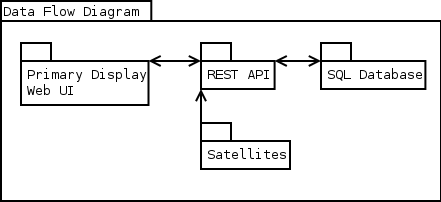
\includegraphics[scale=0.75]{Software/images/DataFlowDiagram.png}
\caption{Data Flow Diagram}
\label{DataFlowDiagram}
\end{figure}

Figure \ref{DataFlowDiagram} shows how various components will be interacting. Notice that the database is not directly accessed by any components, but goes through the REST API instead. This allows us to provide a standard interface should be more-or-less accessible from any programming language or system. This will also allow us to use some well-known security features, such as TLS.

\section{UML Diagrams}

% Any diagrams that can describe the system design
%  Such as inheritance and actors

\section{Potential Problems}

Using open-source libraries requires us to learn them. This is a big problem because of the time constraints on this project, and will require us to spend almost as much time learning as we will be in development (possibly more). This can lead to frustration, especially in light of the fact that we will need to learn the languages in addition to the libraries.

However, using well developed and designed libraries allows us to skip over a good part of the development and planning. We will be able to use extensive API's without taking responsibility for maintaining the software. This will allow us to focus on our product instead of the all the small things that make it up. 

\section{The Backend}

% The backend things
%% Template file for all Software/Hardware modules

% Replace "Name of Module" with the name of this module
\subsection{Authentication}

\subsubsection{Description}

This module describes the architecture of how the backend will manage features related to users and groups (authentication features).

The backend authentication management provided by Django is very robust. It includes user authentication, access control (including groups and individual permissions), administrative panels, and logging of who does what. 

\subsubsection{Program Flow}

The authentication module will be called whenever a user tries to access something. It will verify that the user is logged in, has permissions, and even write a short log message if it is an administrative function.

\subsubsection{Data Flow}

Because this module is not being written by us, it will not be following the standards we are using. Therefore, it will be using the standard Django classes to access database objects instead of going through the REST API. 

While that is not ideal, it should be OK anyway. This part of the Django framework has been tested extensively, in many production environments. There is a low risk that something will not work, and if there is a problem there is a very high chance that upon being reported to the Django project, it will be fixed quickly.

\subsubsection{Potential Problems}

% A list of potentional programs along with suggestions
%  on ways to work around them. Elaborate on why the problem
%  exists

\subsubsection{Sub-modules 1}

% This is a second subsubsection of modules,
%  and should consists of this module broken 
%  down further into components
%% Template file for all Software/Hardware modules

% Replace "Name of Module" with the name of this module
\subsection{The REST API}

\subsubsection{Description}

This module describes the architecture of how the backend will manage features related to providing access to the REST API.

The REST API will provide a \filename{urls.py} file, which will provide a handler for all REST methods.
These could be achieved by simply using the tastypie URL's, which can be generated by calling \filename{include(api\_v1.urls)} in the urlpatterns object.

\subsubsection{Program Flow}

The REST API will be activated by the Django chain when a request comes in for the access to the API, or when another module directly calls functions in the API during their response to a request from the user.

Having each module register itself when the system launches should work, but there may be a problem with things getting registered twice.


\subsubsection{Data Flow}

All data will be returned to the calling client either as a Python dictionary (if called directly from another module), or as JSON, XML, or YAML through a web request (as specified in the query filter using ?format=json).

The REST API will directly access the database.
Initially, tastypie will be dealing with converting the HTTP request to a method on the Django objects.
Django will be generating the SQL that actually gets run, and encapsulating objects in Python classes.


\subsubsection{Potential Problems}

At first, we will be using a prepackaged Django module to help provide the REST API.
This could be problematic because we don't know a lot about the implementation of the API, and if there is a problem, tracking it down could be difficult.

The good news is that django-tastypie is well supported by the community, and source code is liberally commented.
It follows Python commenting standards, and should be fairly easy to navigate.
In addition, members of our team have already used tastypie for projects in both work and recreation.

The most problematic bit about using tastypie for the initial run-through is the compatibility problems it has with Backbone.js.
However, the community has developed an addition to Backbone to help deal with this.
It is called Backbone-tastypie.
It is a simple modification to the Backbone sync operations that allows it to communicate with a standard tastypie REST API.

When the web server is launched, it initialized all modules by calling their \filename{\_\_init\_\_.py} file.
In this file, each module can register themselves with the API.
This will allow all modules to be self-contained, which is ideal in that it will allow us to upgrade one module without breaking everything else.

Early experiments indicate that the \filename{\_\_init\_\_.py} file is called twice during the loading of the system.
This could be solved a number of ways, or it might not even be a problem. 
It's very possible the first time the module is loaded it is just being checked for syntax and compiled, then the program is restarting with the compiled files.

%% Template file for all Software/Hardware modules

% Replace "Name of Module" with the name of this module
\subsection{Satellite}

\subsubsection{Description}

This module describes the architecture of how the back end will manage features related to managing Satellites. 

The Satellite Management back end is in control of maintaining the information in the database pertaining to Satellites. 
The back end will also generate the framework for the web pages. 
It will pass the basic form of the Satellite Management page to the front end to be filled in with additional formatting. 

\subsubsection{Program Flow}

The back end Satellite Management module will be activated by a request from the front end Satellite Management. 
This module will complete the request by adding information to the SQL database or querying said database for specific data. 

\subsubsection{Data Flow}

The Data Flow will behave in much the same manner as the Program Flow. 
The back end Satellite Management module will receive data from the Satellite Management front end via the REST API. 
This includes data that needs to be changed in the database, and requests for data. 
This module will then modify or query the database as needed, 
returning the requested data or a confirmation of modification to the front end through the REST API. 

\subsubsection{Sub-modules}
Communication with the Satellites:\\
This modules serves as an interface and a form listnener. 
It will receive POSTed commands for dispatch to the ZigBee network via a serial-port connected ZigBee. 
It will also receive the incoming data from the ZigBee network and store it in the Database. 
The data will consist of the current and voltage readings from each Satellite on the network. 

%% Template file for all Software/Hardware modules

% Replace "Name of Module" with the name of this module
\subsection{Devices}

\subsubsection{Description}

This module describes the architecture of how the back end will manage features related to Device Management.

The Device Management back end will be in charge of maintaining the database with information pertaining to the Devices. 

 

\subsubsection{Program Flow}

The user will be presented with the option to add, edit, or disable a device. 
Adding a device allows the user to name the new device and associate it with a specific Satellite. 
Editing a device allows the user to change the Satellite associated with the device. 
The user will not have the option to edit the name of the device once it has been created in order to maintain consistant data with each device. 
Disabling a device will remove it from 

% Insert a flow chart here with a high-level look
%  at the states this part of the system goes through

\subsubsection{Data Flow}

The back end Device Management module will receive data from the Device Management front end via the REST API. 
This includes data that needs to be changed in the database, and requests for data. 
This module will then modify or query the database as needed, 
returning the requested data or a confirmation of modification to the front end through the REST API. 


% Describe where data goes and comes from in this subsubsection
% Flow charts are encouraged

\subsubsection{UML Diagrams}

% Any diagrams that can describe the system design
%  Such as inheritance and actors

\subsubsection{Potential Problems}

% A list of potentional programs along with suggestions
%  on ways to work around them.
Elaborate on why the problem
%  exists

\subsubsection{Sub-modules 1}

% This is a second subsubsection of modules,
%  and should consists of this module broken 
%  down further into components
%% Template file for all Software/Hardware modules

% Replace "Name of Module" with the name of this module
\subsection{Power Bill Guestimator}

\subsubsection{Description}

This module describes the architecture of how the backend will manage features related to the power bill guestimator.

\subsubsection{Program Flow}

% Insert a flow chart here with a high-level look
%  at the states this part of the system goes through

\subsubsection{Data Flow}

% Describe where data goes and comes from in this subsubsection
% Flow charts are encouraged

\subsubsection{UML Diagrams}

% Any diagrams that can describe the system design
%  Such as inheritance and actors

\subsubsection{Potential Problems}

% A list of potentional programs along with suggestions
%  on ways to work around them. Elaborate on why the problem
%  exists

\subsubsection{Sub-modules 1}

% This is a second subsubsection of modules,
%  and should consists of this module broken 
%  down further into components
%% Template file for all Software/Hardware modules

% Replace "Name of Module" with the name of this module
\subsection{Factory Reset}

\subsubsection{Description}

This module describes the architecture of how the backend will manage features related to the factory reset.
The factory reset will restore everything to the exact same way it was when the system came out of the "factory".
This means that all data will be wiped, and custom modifications will be wiped, and any software upgrade will be wiped.

\subsubsection{Program Flow}

This function will be invoked either through a call passed down from the web interface (it will be handled by the \ac{REST} \ac{API}, and the call will be intercepted and result in an action) or by a program picking up on the push of the physical factory-reset button.

\subsubsection{Data Flow}

Doing the factory restore will involve a good bit of trickery. 
First, we will need to put a partition on the disk that stores all the files that make up the "live" running system. 
This might be best done by simply putting a tarball and a script on a small partition at the end of the disk. 
The script will be responsible for wiping the primary partition, re-creating it, and extracting the tarball.

Getting the system to boot into the "restore" mode will involve modifying grub settings on the fly. 
We can do this, and it shouldn't be too hard, but it feels like a really bad idea.

After the machine is in recovery mode, something will need to launch the script to do the restore.
This shouldn't be too difficult if just use an old-school \filename{rc.conf} script or something of the sort.
The script will also restore grub, so we don't have to worry about returning that to it's old good state.

\subsubsection{Potential Problems}

One of the biggest risks here is failing to boot into the restore partition and ruining our grub configuration.
This would cause the customer to need to send us back the unit, we would have to flash it, and send it back.
If we can get this feature working however, we will not have to worry so much about breaking the web UI by accident.


\section{The Frontend}

% And these are the frontend things
%% Template file for all Software/Hardware modules

% Replace "Name of Module" with the name of this module
\subsection{Authentication}

\subsubsection{Description}

This module describes the architecture of how the frontend will create pages that allow the user to manage user and groups.

The authentication front end will consist of both the "login" page, and the user management pages. These pages either post directly to the server using standard form-submission methods (ie, not Ajax) or by using AJAX (if we have time to recreate the entire management system). 

\subsubsection{Program Flow}

The user will first be presented with a login screen, which will take two pieces of information:
\begin{itemize}
 \item Username - The user's username
 \item Password - The user's password
\end{itemize}

After these two pieces of information have been verified (ie, that password belongs to that user), the user will be logged in.

From here, the user has all kinds of options. The only ones that are interesting to this module is the settings panel, which includes a link to the user administration panel. The user administration panel will, initially, be a themed Django-admin view. Time permitting, this may be recreated to be a AJAX type interface.

\subsubsection{Data Flow}

All data will be sent to the server through POST requests, not through the REST API. This will allow us to skip over this module almost entirely. This is not consistent with everything else, and will need to be remade later on if there is time.

\subsubsection{Potential Problems}

Themeing the admin interface to match our site will be tricky. At best, it will involve telling Django to include some extra stylesheets or using a different template. At worst, it will involve modifying the Django stylesheets directly. Either option works, but due to version control it would greatly preferred to be able to tell Django what styles to use.

%% Template file for all Software/Hardware modules

% Replace "Name of Module" with the name of this module
\subsection{Satellite}

\subsubsection{Description}

This module describes the architecture of how the frontend will create pages that allow the user to add, remove, and modify Satellites associated with the system.

\subsubsection{Program Flow}

The Satellite Management front end consists of the Satellite Management page. 
This page leads to a set-up wizard for syncing new Satellites with the Server. 
The wizard walks the user through instructions 

% Insert a flow chart here with a high-level look
%  at the states this part of the system goes through

\subsubsection{Data Flow}

% Describe where data goes and comes from in this subsubsection
% Flow charts are encouraged

\subsubsection{UML Diagrams}

% Any diagrams that can describe the system design
%  Such as inheritance and actors

\subsubsection{Potential Problems}

% A list of potentional programs along with suggestions
%  on ways to work around them.
Elaborate on why the problem
%  exists

\subsubsection{Sub-modules 1}

% This is a second subsubsection of modules,
%  and should consists of this module broken 
%  down further into components
%% Template file for all Software/Hardware modules

% Replace "Name of Module" with the name of this module
\subsection{Devices}

\subsubsection{Description}

This module describes the architecture of how the frontend will create pages that allow the user to manage devices in the system.

\subsubsection{Program Flow}

% Insert a flow chart here with a high-level look
%  at the states this part of the system goes through

\subsubsection{Data Flow}

% Describe where data goes and comes from in this subsubsection
% Flow charts are encouraged

\subsubsection{UML Diagrams}

% Any diagrams that can describe the system design
%  Such as inheritance and actors

\subsubsection{Potential Problems}

% A list of potentional programs along with suggestions
%  on ways to work around them. Elaborate on why the problem
%  exists

\subsubsection{Sub-modules 1}

% This is a second subsubsection of modules,
%  and should consists of this module broken 
%  down further into components
%% Template file for all Software/Hardware modules

% Replace "Name of Module" with the name of this module
\subsection{Frontend - View Data}

\subsubsection{Description}

This module describes the architecture of how the frontend will create pages that allow the user to view various pieces of data in various formats.

The View Data front end is responsible for providing the user with data regarding each device and device group. 
It will 

\subsubsection{Program Flow}



% Insert a flow chart here with a high-level look
%  at the states this part of the system goes through

\subsubsection{Data Flow}

% Describe where data goes and comes from in this subsubsection
% Flow charts are encouraged

\subsubsection{UML Diagrams}

% Any diagrams that can describe the system design
%  Such as inheritance and actors

\subsubsection{Potential Problems}

% A list of potentional programs along with suggestions
%  on ways to work around them. Elaborate on why the problem
%  exists

\subsubsection{Sub-modules 1}

% This is a second subsubsection of modules,
%  and should consists of this module broken 
%  down further into components
%% Template file for all Software/Hardware modules

% Replace "Name of Module" with the name of this module
\subsection{Power Bill Guestimator}

\subsubsection{Description}

This module describes the architecture of how the frontend will create pages that allow the user to view guestimates of their monthly power bill, in various scenarios.

\subsubsection{Program Flow}

% Insert a flow chart here with a high-level look
%  at the states this part of the system goes through

\subsubsection{Data Flow}

% Describe where data goes and comes from in this subsubsection
% Flow charts are encouraged

\subsubsection{UML Diagrams}

% Any diagrams that can describe the system design
%  Such as inheritance and actors

\subsubsection{Potential Problems}

% A list of potentional programs along with suggestions
%  on ways to work around them. Elaborate on why the problem
%  exists

\subsubsection{Sub-modules 1}

% This is a second subsubsection of modules,
%  and should consists of this module broken 
%  down further into components
%% Template file for all Software/Hardware modules

% Replace "Name of Module" with the name of this module
\section{Factory Reset}

\subsubsection{Description}

This module describes the architecture of how the frontend will create pages that allow the user to reset the system back to factory default settings.

\subsubsection{Program Flow}

% Insert a flow chart here with a high-level look
%  at the states this part of the system goes through

\subsubsection{Data Flow}

% Describe where data goes and comes from in this subsubsection
% Flow charts are encouraged

\subsubsection{UML Diagrams}

% Any diagrams that can describe the system design
%  Such as inheritance and actors

\subsubsection{Potential Problems}

% A list of potentional programs along with suggestions
%  on ways to work around them. Elaborate on why the problem
%  exists

\subsubsection{Sub-modules 1}

% This is a second subsubsection of modules,
%  and should consists of this module broken 
%  down further into components

% This is a second section of modules,
%  and should consists of this module broken 
%  down further into components

